\section{Existing Systems Analysis}

\subsection{Introduction}

The sustained growth of digital commerce and smart mobility services has generated significant market demand for online vehicle rental platforms. Incumbent systems --- ranging from large aggregators to local operators --- provide varying degrees of vehicle search, booking, payment integration, and fleet management capability. However, as the analysis below demonstrates, most existing platforms exhibit persistent limitations in owner-renter communication transparency, trust verification, pricing flexibility, and support for the emerging P2P sharing model. These gaps directly motivate the design decisions embedded in LuxeWay.

\subsection{Existing Vehicle Rental Systems}

\subsubsection{Grab Rentals}

\begin{figure}[htbp]
    \centering
    \begin{minipage}[b]{0.32\textwidth}
        \centering
        
\includegraphics[width=\textwidth]{grab1.png}
    \end{minipage}
    \hfill
    \begin{minipage}[b]{0.32\textwidth}
        \centering
        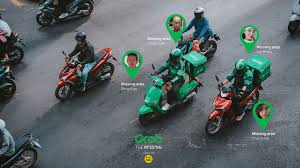
\includegraphics[width=\textwidth]{grab2.jpg}
    \end{minipage}
    \hfill
    \begin{minipage}[b]{0.32\textwidth}
        \centering
        
\includegraphics[width=\textwidth]{grab3.jpg}
    \end{minipage}
    \caption{Grab Rentals Interface}
    \label{fig:grab_interface}
\end{figure}

Grab Rentals is a transportation service platform embedded within the broader Grab super-app ecosystem, enabling users to book vehicles through a unified mobile interface. The platform prioritizes frictionless transactions and rapid booking confirmation within an established consumer base.

\begin{itemize}
    \item \textbf{Strengths:} Streamlined booking workflow with minimal user steps; tightly integrated online payment system; real-time booking confirmation and push notifications; extensive brand trust and large existing user base; strong mobile-first experience optimized for Southeast Asian markets.

    \item \textbf{Weaknesses:} Rigid rental duration options with limited customization; vehicle specification detail is often insufficient for informed decision-making; review and dispute transparency is constrained by the platform's black-box design; heavy dependency on the mobile application with no equivalent web interface; pricing complexity increases significantly during peak demand periods.

    \item \textbf{Analysis:} Grab Rentals delivers a highly efficient transactional experience optimized for speed and convenience. However, the platform is architecturally designed around Grab's B2C transportation model rather than a P2P asset-sharing paradigm. As a result, mechanisms for owner-renter communication, vehicle trust evaluation, and flexible listing customization are notably underdeveloped compared to dedicated rental marketplace standards.
\end{itemize}

\subsubsection{Traveloka Car Rental}

\begin{figure}[htbp]
    \centering
    \begin{minipage}[b]{0.45\textwidth}
        \centering
        
\includegraphics[width=\textwidth]{tv1.jpg}
    \end{minipage}
    \hfill
    \begin{minipage}[b]{0.45\textwidth}
        \centering
        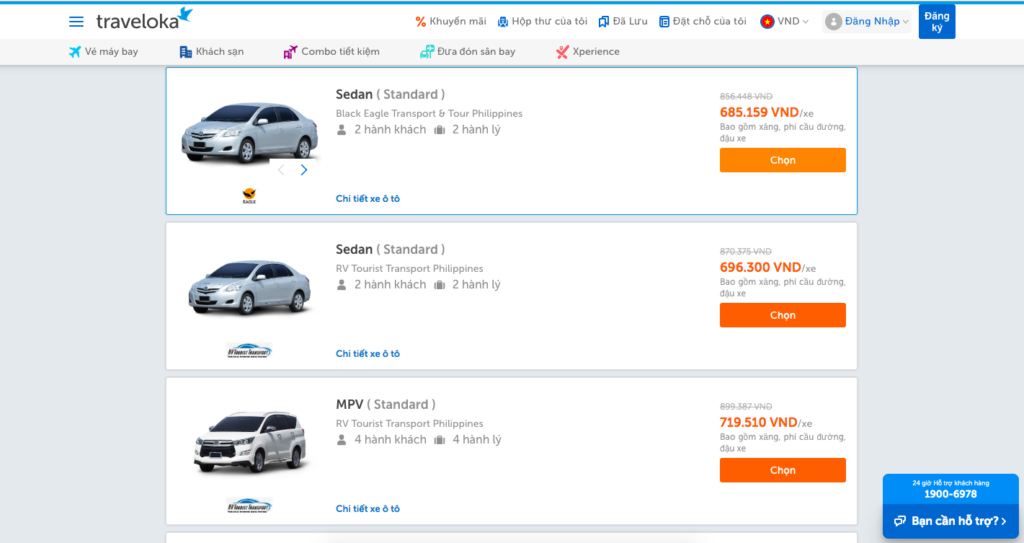
\includegraphics[width=\textwidth]{tv2.png}
    \end{minipage}
    \caption{Traveloka Car Rental Interface}
    \label{fig:traveloka_interface}
\end{figure}

Traveloka Car Rental is a vertical within the Traveloka travel super-platform, offering vehicle rental services tightly bundled with flight, hotel, and tourism booking capabilities. The service targets travelers seeking integrated itinerary management rather than standalone vehicle rental.

\begin{itemize}
    \item \textbf{Strengths:} Deeply integrated travel booking ecosystem enabling bundle pricing; diverse vehicle category coverage across major Vietnamese cities; reliable payment processing with consumer protection guarantees; established brand reputation across Southeast Asia; multi-criteria search and filtering tools.

    \item \textbf{Weaknesses:} Interface complexity increases cognitive load for users seeking a standalone rental experience; no direct messaging channel between renter and vehicle provider; a subset of bookings requires manual back-office confirmation, introducing operational latency; identity and review verification mechanisms are opaque to consumers.

    \item \textbf{Analysis:} Traveloka's rental vertical succeeds as a convenience layer for travelers already embedded in its ecosystem, but falls short as a dedicated P2P rental marketplace. The absence of direct owner-renter communication and the opacity of the review verification process represent material gaps relative to a trust-first rental platform such as LuxeWay.
\end{itemize}

\subsubsection{Local Vehicle Rental Websites}

\begin{figure}[htbp]
    \centering
    \begin{minipage}[b]{0.45\textwidth}
        \centering
        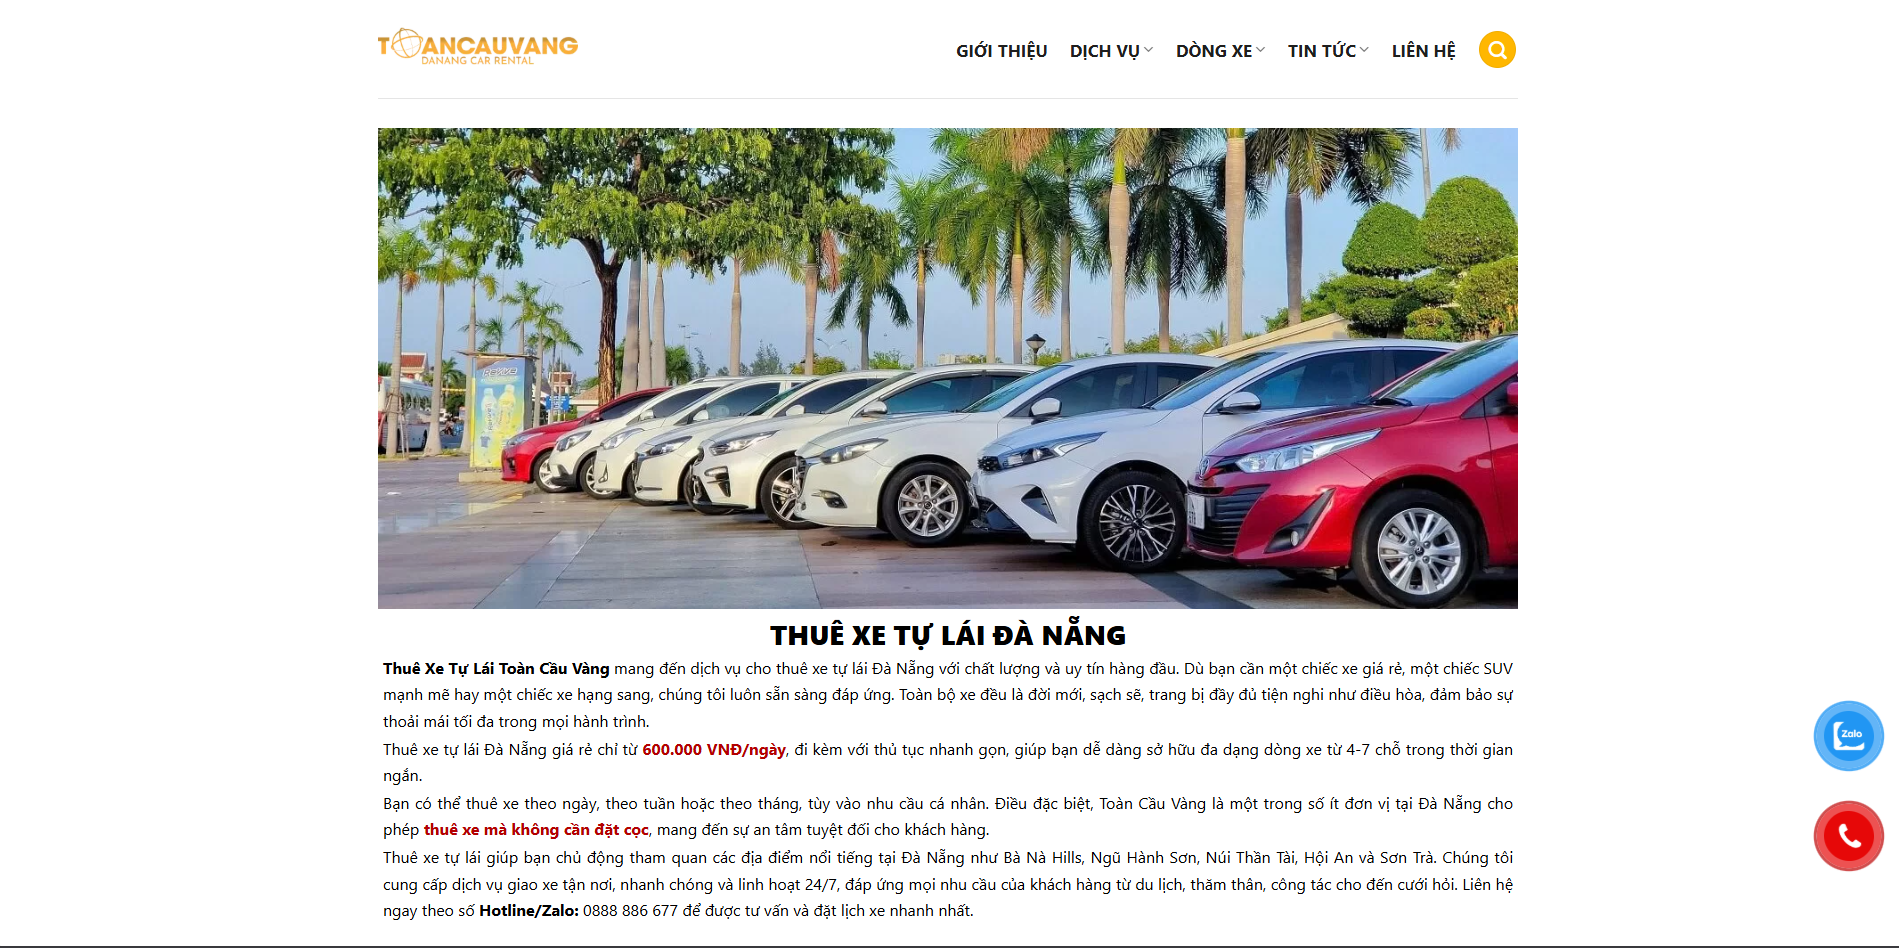
\includegraphics[width=\textwidth]{lcr1.png}
    \end{minipage}
    \hfill
    \begin{minipage}[b]{0.45\textwidth}
        \centering
        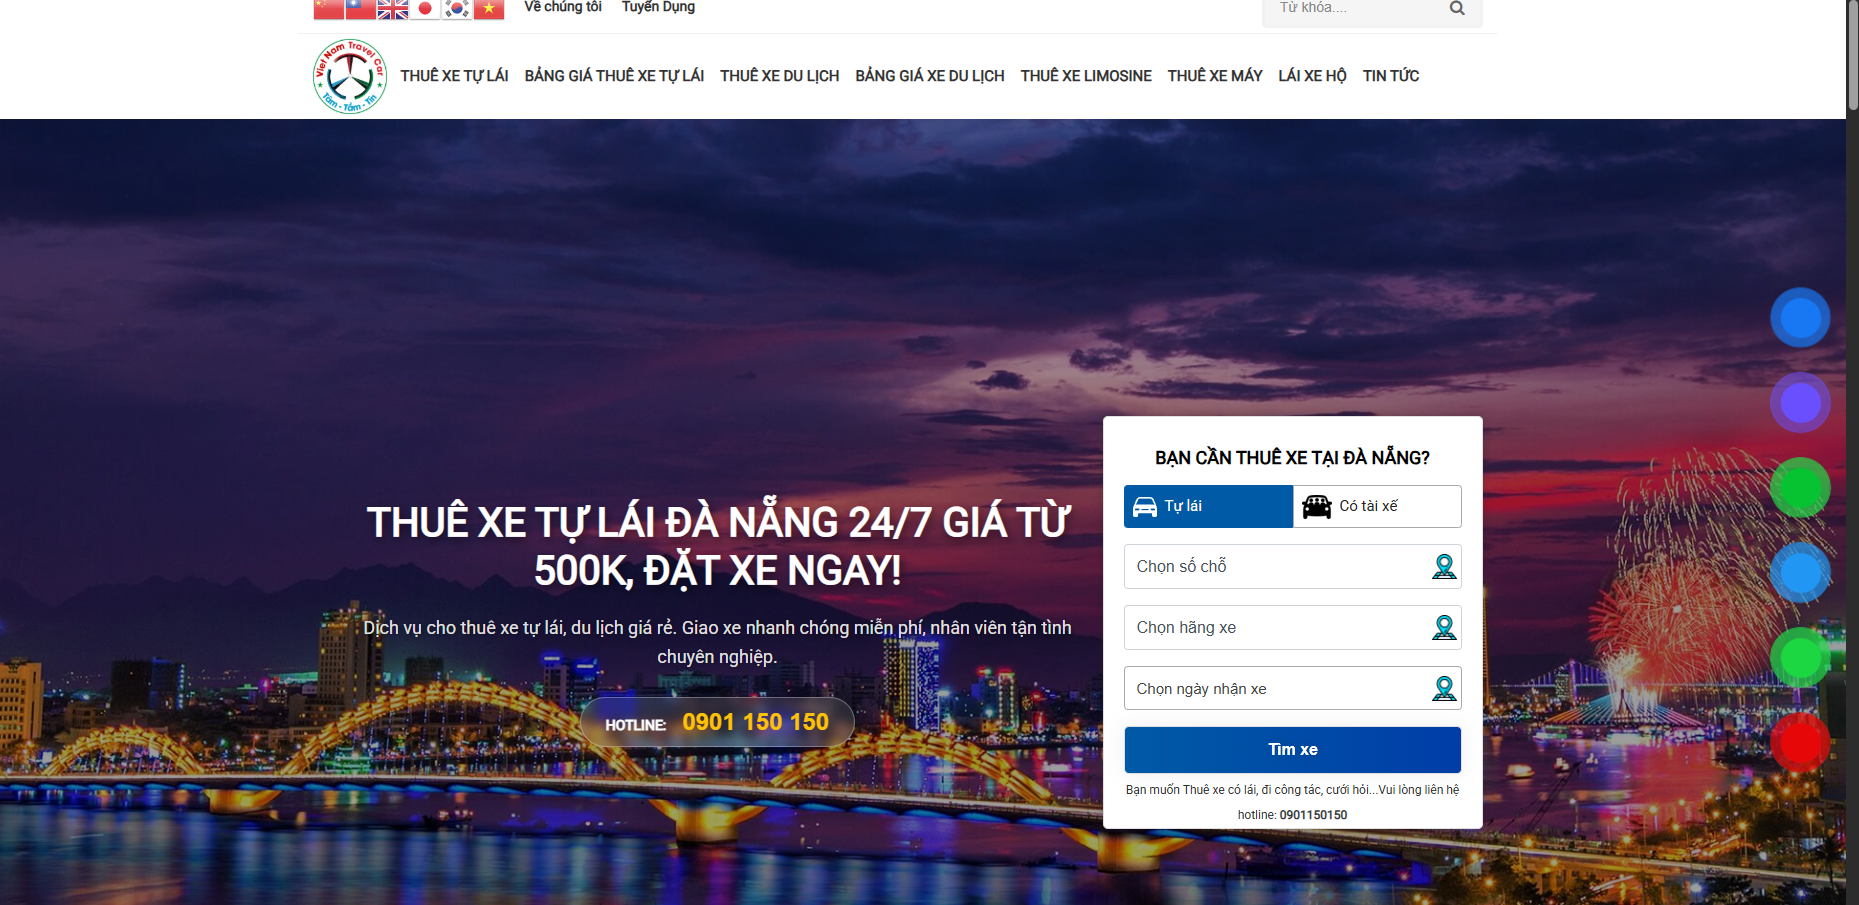
\includegraphics[width=\textwidth]{lcr2.png}
    \end{minipage}
    \caption{Local Vehicle Rental Website Examples}
    \label{fig:local_rental}
\end{figure}

Independent local rental operators in Vietnam typically maintain bespoke booking websites with varying levels of technical sophistication. These systems generally provide basic vehicle listing, contact-based booking requests, and manual payment confirmation.

\begin{itemize}
    \item \textbf{Strengths:} Flexible pricing and negotiation; personalized customer support; simpler booking workflows suited to repeat customers.

    \item \textbf{Weaknesses:} Weak authentication and security mechanisms; outdated and non-responsive UI/UX design; limited payment gateway integration; absence of digital contract or booking audit trail; no verified review infrastructure; poor scalability beyond a single operator.

    \item \textbf{Analysis:} While local rental websites offer flexibility and direct owner interaction, they consistently lack the standardized security practices, scalable booking workflows, digital contract support, and trust infrastructure required for a credible P2P marketplace. Their fragmented nature creates an unmet market need for a consolidated, trustworthy rental platform.
\end{itemize}

\subsection{Comparative Summary}

\begin{table*}[ht]
\centering
\caption{Comparative Summary of Existing Rental Systems}
\label{tab:existing_systems}
\begin{tabular}{p{3.2cm} p{6cm} p{6cm}}
\toprule
\textbf{System} & \textbf{Key Strengths} & \textbf{Key Weaknesses} \\
\midrule
Grab Rentals & Fast booking; large user base; integrated payments & No web interface; rigid options; limited trust transparency \\
Traveloka Car Rental & Broad vehicle range; trusted brand; bundle pricing & No owner-renter chat; opaque reviews; manual confirmation \\
Local Rental Websites & Flexible pricing; personalized service & Weak security; no digital contracts; no verified reviews \\
\bottomrule
\end{tabular}
\end{table*}

\subsection{Implications for LuxeWay}

The analysis of existing platforms reveals a consistent set of structural limitations that LuxeWay is specifically designed to address:

\begin{itemize}
    \item \textbf{Owner-renter communication gap} $\rightarrow$ WebSocket real-time chat (STOMP/SockJS)
    \item \textbf{Single-dimension or opaque ratings} $\rightarrow$ Five-dimension review model per verified booking
    \item \textbf{No direct P2P listing control} $\rightarrow$ Owner self-service listing with full specification, image, and pricing management
    \item \textbf{Limited payment localization} $\rightarrow$ VNPay gateway + LuxeWallet with Vietnamese bank and e-wallet support
    \item \textbf{No digital rental contracts} $\rightarrow$ Auto-generated PDF contract (iText) on booking confirmation
    \item \textbf{Manual or absent KYC} $\rightarrow$ Structured document upload and admin-driven verification workflow
    \item \textbf{Poor mobile-web consistency} $\rightarrow$ Responsive React SPA optimized for both desktop and mobile browsers
\end{itemize}
